\documentclass[aspectratio=169, 10pt]{beamer}

\usetheme{Madrid}
\usecolortheme{whale}

\usepackage{amsmath, amssymb, amsthm}
\usepackage{bm}
\usepackage{tikz}
\usetikzlibrary{arrows.meta, positioning, shapes.geometric}
\usepackage{booktabs}
\usepackage{xcolor}

% Custom colors
\definecolor{darkblue}{RGB}{0,51,102}
\definecolor{darkred}{RGB}{153,0,0}
\definecolor{darkgreen}{RGB}{0,102,51}
\definecolor{lightblue}{RGB}{220,235,245}
\definecolor{lightyellow}{RGB}{255,250,220}
\definecolor{lightgreen}{RGB}{220,245,220}

\setbeamercolor{palette primary}   {bg=darkblue, fg=white}
\setbeamercolor{palette secondary} {bg=darkblue!80, fg=white}
\setbeamercolor{palette tertiary}  {bg=darkblue!60, fg=white}
\setbeamercolor{palette quaternary}{bg=darkblue, fg=white}
\setbeamercolor{frametitle}        {bg=darkblue, fg=white}
\setbeamercolor{title}             {fg=white}

% Notation shortcuts
\newcommand{\Rbar}{\bar{R}}
\newcommand{\Phat}{\hat{P}}
\newcommand{\Lhat}{\hat{\Lambda}}
\newcommand{\Qhat}{\hat{Q}}
\newcommand{\Wone}{W^{(1)}}
\newcommand{\Wzero}{W^{(0)}}
\newcommand{\Pw}{P_{W^{(1)}}}
\newcommand{\norm}[1]{\left\|#1\right\|_F}

%
%===================================================================================================
%
% Title page information

\author{Giovanni Della Lunga\\{\footnotesize giovanni.dellalunga@unibo.it}}
\title{Chapter 2\\Factor Models and Dimensionality Reduction}
\subtitle{Appendix 1 - Why the Optimal Decoder Satisfies $\Wone = \Phat A$} % (optional)
\setbeamercovered{transparent} 
\institute{Advanced Topics in Artificial Intelligence} 
\date{Bologna - March, 2026} 
%
%===================================================================================================
%
\begin{document}
%
%===================================================================================================
%
\begin{frame}
\titlepage
\end{frame}
%
%===================================================================================================
%
\begin{frame}{Roadmap}
\tableofcontents
\end{frame}
%
%..................................................................
%
\begin{frame}{The Linear Autoencoder: Setup}

We train a one-hidden-layer autoencoder with \textbf{linear} activation on the
$N \times T$ matrix of demeaned returns $\Rbar$.

\medskip
After two preliminary steps (shown in the full proof):
\begin{enumerate}
  \item The \textbf{bias terms} absorb the mean return $\bar{r}$ and drop out
  \item The \textbf{optimal encoder} $\Wzero$ equals the pseudoinverse of the decoder $\Wone$:
        $$\Wzero = \bigl(\Wone{}'\Wone\bigr)^{-1}\Wone{}'$$
\end{enumerate}

\medskip
Substituting $\Wzero$ back, the optimization reduces to:

\begin{block}{The Core Problem}
$$\min_{\Wone} \; \norm{\Rbar - \Pw \Rbar}^2$$
where $\Pw = \Wone\bigl(\Wone{}'\Wone\bigr)^{-1}\Wone{}'$ is the
\textbf{orthogonal projector} onto the column space of $\Wone$.
\end{block}

\medskip
\textbf{Goal of this presentation:} show that the solution to this problem is
$$\boxed{\Wone = \Phat A}$$
for any invertible $K\times K$ matrix $A$, where $\Phat$ are the left singular
vectors of $\Rbar$.

\end{frame}

% -------------------------------------------------------
\section{Key Tools}

\begin{frame}{Tool 1 — The SVD of $\Rbar$}

The \textbf{Singular Value Decomposition} of $\Rbar \in \mathbb{R}^{N\times T}$ (truncated to rank $K$) is:

$$\Rbar = \Phat\Lhat\Qhat + U$$

\begin{center}
\begin{tabular}{cll}
\toprule
\textbf{Object} & \textbf{Dimension} & \textbf{Property} \\
\midrule
$\Phat$ & $N\times K$ & orthonormal columns: $\Phat{}'\Phat = I_K$ \\
$\Lhat$ & $K\times K$ & diagonal, $\sigma_1\geq\cdots\geq\sigma_K>0$ \\
$\Qhat$ & $K\times T$ & orthonormal rows: $\Qhat\Qhat{}'= I_K$ \\
$U$     & $N\times T$ & residual \\
\bottomrule
\end{tabular}
\end{center}

\bigskip
\begin{alertblock}{Crucial orthogonality property}
The residual $U$ is \textbf{orthogonal to the column space of $\Phat$}:
$$\Phat{}'U = 0$$
This follows directly from the construction of the SVD.
\end{alertblock}

\end{frame}

% -------------------------------------------------------
\begin{frame}{Tool 2 — The Eckart–Young–Mirsky Theorem}

\begin{block}{Theorem (Eckart–Young–Mirsky, 1936)}
Among all $N\times T$ matrices of rank at most $K$, the one closest to $\Rbar$
in Frobenius norm is its truncated SVD:
$$\Rbar^{(K)} = \Phat\Lhat\Qhat$$
That is, for any matrix $M$ with $\mathrm{rank}(M)\leq K$:
$$\norm{\Rbar - \Phat\Lhat\Qhat} \leq \norm{\Rbar - M}$$
\end{block}

\bigskip
\textbf{Why does this apply here?}

The reconstruction $\Pw\Rbar$ has rank at most $K$ (the projector $\Pw$ has rank $K$).
So our minimization problem is exactly a \emph{best rank-$K$ approximation} problem:

$$\min_{\Wone} \norm{\Rbar - \Pw\Rbar}^2 \quad\Longleftrightarrow\quad
  \min_{M:\,\mathrm{rank}(M)\leq K} \norm{\Rbar - M}^2$$

and Eckart–Young tells us the solution is $M^* = \Phat\Lhat\Qhat$.

\end{frame}

% -------------------------------------------------------
\begin{frame}{Tool 3 — Projectors and Subspaces}

\begin{block}{Key fact}
An orthogonal projector $P$ onto a subspace $\mathcal{S}$ is \textbf{uniquely
determined by $\mathcal{S}$}, not by the particular basis chosen for $\mathcal{S}$.
\end{block}

\medskip
Consequence: two matrices $W$ and $\tilde{W}$ generate the \textbf{same projector}
if and only if they have the \textbf{same column space}:
$$P_W = P_{\tilde{W}} \iff \mathrm{col}(W) = \mathrm{col}(\tilde{W})$$

\medskip
\begin{exampleblock}{Example}
Let $\Phat$ have orthonormal columns and $A$ be any $K\times K$ invertible matrix.
Then $\mathrm{col}(\Phat A) = \mathrm{col}(\Phat)$, because multiplying on the right
by an invertible matrix is just a change of basis within the same subspace.

Therefore: $P_{\Phat A} = P_{\Phat} = \Phat\Phat'$.
\end{exampleblock}

\end{frame}

% -------------------------------------------------------
\section{The Proof}

\begin{frame}{Step 1 — Apply Eckart–Young}

From the theorem, the \textbf{optimal reconstruction} is:

$$P_{\Wone}^*\,\Rbar = \Phat\Lhat\Qhat$$

So we need to find $\Wone$ such that:

$$\Pw\,\Rbar = \Phat\Lhat\Qhat$$

\medskip
\textbf{The key rewriting:} we claim that

\begin{alertblock}{Claim}
$$\Phat\Lhat\Qhat = \Phat\Phat'\Rbar$$
\end{alertblock}

\medskip
If this claim is true, then the condition becomes:
$$\Pw\,\Rbar = \Phat\Phat'\Rbar$$

which suggests that $\Pw = \Phat\Phat'$, i.e.\ the optimal projector is the
projection onto the column space of $\Phat$.

\medskip
Let us prove the claim.

\end{frame}

% -------------------------------------------------------
\begin{frame}{Step 2 — Why $\Phat\Lhat\Qhat = \Phat\Phat'\Rbar$ (The Key Calculation)}

Start from the SVD decomposition of $\Rbar$:

$$\Rbar = \underbrace{\Phat\Lhat\Qhat}_{\text{rank-}K\text{ part}} + \underbrace{U}_{\text{residual}}$$

Apply $\Phat\Phat'$ to both sides:

$$\Phat\Phat'\Rbar = \Phat\Phat'(\Phat\Lhat\Qhat) + \Phat\Phat' U$$

\medskip
\textbf{First term:}
$$\Phat\Phat'(\Phat\Lhat\Qhat) = \Phat\underbrace{(\Phat'\Phat)}_{= I_K}\Lhat\Qhat = \Phat\Lhat\Qhat$$

\textbf{Second term:}
$$\Phat\Phat' U = \Phat\underbrace{(\Phat' U)}_{= 0}\;= 0$$

because $\Phat' U = 0$ (orthogonality property of the SVD).

\medskip
\begin{exampleblock}{Result}
$$\Phat\Phat'\Rbar = \Phat\Lhat\Qhat + 0 = \Phat\Lhat\Qhat \qquad \checkmark$$
\end{exampleblock}

\medskip
\small \textit{Note: $\bar{R}$ does not ``disappear'' — it gets absorbed into the SVD structure.
The residual $U$ vanishes because it is orthogonal to $\hat P$ by construction.}

\end{frame}

% -------------------------------------------------------
\begin{frame}{Step 3 — Identify the Optimal Projector}

We have shown that the optimal reconstruction satisfies:

$$\Pw^*\,\Rbar = \Phat\Phat'\Rbar$$

\bigskip
\textbf{Does this mean $\Pw^* = \Phat\Phat'$?}

\medskip
Yes — but we need to be careful. The equation $\Pw\Rbar = \Phat\Phat'\Rbar$ must
hold for \emph{all} configurations of returns, not just for the specific $\Rbar$ in
our sample. Since the projector is a property of the model (not of the data), we can
identify:

\begin{block}{Optimal Projector}
$$\Pw^* = \Phat\Phat'$$
\end{block}

\medskip
This is the orthogonal projector onto the \textbf{K-dimensional subspace spanned by
the columns of $\Phat$} (the top-$K$ left singular vectors of $\Rbar$).

\end{frame}

% -------------------------------------------------------
\begin{frame}{Step 4 — From the Projector to $\Wone$}

We need: which matrices $\Wone$ generate the projector $\Phat\Phat'$?

\medskip
Recall that $\Pw = \Wone(\Wone{}'\Wone)^{-1}\Wone{}'$ is the projector onto
$\mathrm{col}(\Wone)$. Since a projector uniquely determines its subspace:

$$\Pw = \Phat\Phat' \iff \mathrm{col}(\Wone) = \mathrm{col}(\Phat)$$

\medskip
\textbf{Which $N\times K$ matrices have the same column space as $\Phat$?}

Exactly those of the form $\Phat A$ for some \textbf{invertible} $K\times K$ matrix $A$:
\begin{itemize}
  \item $\mathrm{col}(\Phat A) = \mathrm{col}(\Phat)$ because $A$ invertible $\Rightarrow$
        $A$ is a change of basis within $\mathbb{R}^K$
  \item Conversely, any matrix with $\mathrm{col}(\Wone) = \mathrm{col}(\Phat)$ can be
        written as $\Phat A$ for some invertible $A$
\end{itemize}

\bigskip
\begin{alertblock}{Conclusion}
$$\boxed{\Wone = \Phat A \quad \text{for any invertible } K\times K \text{ matrix } A}$$
\end{alertblock}

\end{frame}

% -------------------------------------------------------
\section{Why $A$ Does Not Matter}

\begin{frame}{The Rotation $A$ Cancels Out}

One might worry: if there are infinitely many solutions $\Wone = \Phat A$, is the
model ill-defined?

\medskip
\textbf{No} — because $A$ cancels in every economically relevant quantity.

\medskip
\textbf{Reconstruction:}
$$\Pw\Rbar = \Phat\Phat'\Rbar = \Phat\Lhat\Qhat \quad \text{(independent of } A\text{)}$$

\medskip
\textbf{Optimal encoder} (from Step 2 of the full proof):
$$\Wzero = (\Wone{}'\Wone)^{-1}\Wone{}' = A^{-1}\Phat{}'$$

\medskip
\textbf{Estimated factors:}
$$\hat{F} = \Wzero\Rbar = A^{-1}\Phat{}'\Rbar = A^{-1}\Lhat\Qhat$$

\medskip
\textbf{Fitted returns} ($A$ cancels explicitly):
$$\Wone\hat{F} = (\Phat A)(A^{-1}\Lhat\Qhat) = \Phat\Lhat\Qhat \quad \checkmark$$

\begin{exampleblock}{Analogy}
Choosing $A$ is like choosing Fahrenheit vs.\ Celsius: the temperature (the factor
space) is the same; only the coordinate system changes.
\end{exampleblock}

\end{frame}

% -------------------------------------------------------
\section{Summary}

\begin{frame}{Proof at a Glance}

\begin{center}
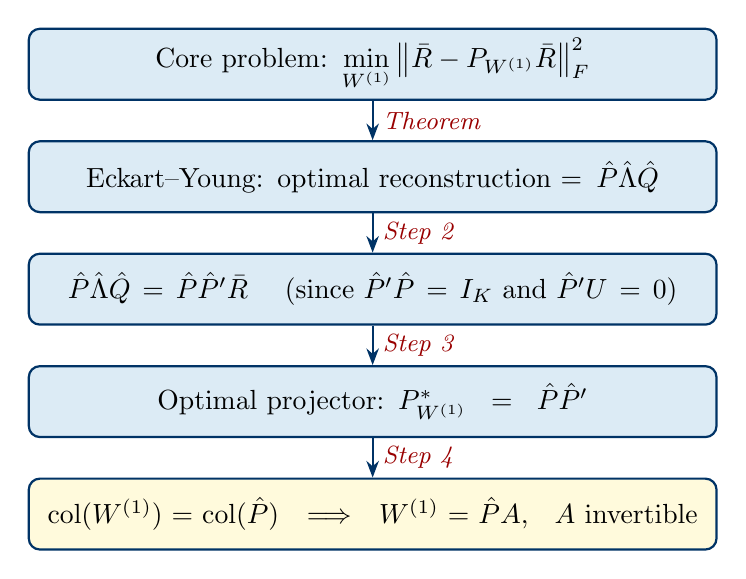
\begin{tikzpicture}[
  box/.style={rectangle, rounded corners, draw=darkblue, thick,
              fill=lightblue, text width=8.5cm, align=center, minimum height=0.9cm},
  arrow/.style={-{Stealth[length=6pt]}, thick, darkblue},
  label/.style={font=\small\itshape, text=darkred}
]
\node[box] (start) {Core problem: $\displaystyle\min_{\Wone}\norm{\Rbar-\Pw\Rbar}^2$};
\node[box, below=0.5cm of start] (ey)
      {Eckart--Young: optimal reconstruction $= \Phat\Lhat\Qhat$};
\node[box, below=0.5cm of ey] (claim)
      {$\Phat\Lhat\Qhat = \Phat\Phat'\Rbar$ \quad (since $\Phat'\Phat=I_K$ and $\Phat'U=0$)};
\node[box, below=0.5cm of claim] (proj)
      {Optimal projector: $\Pw^* = \Phat\Phat'$};
\node[box, fill=lightyellow, below=0.5cm of proj] (sol)
      {$\mathrm{col}(\Wone)=\mathrm{col}(\Phat)$\quad$\Longrightarrow$\quad
       $\Wone = \Phat A$, \; $A$ invertible};

\draw[arrow] (start) -- node[label, right]{Theorem} (ey);
\draw[arrow] (ey)    -- node[label, right]{Step 2} (claim);
\draw[arrow] (claim) -- node[label, right]{Step 3} (proj);
\draw[arrow] (proj)  -- node[label, right]{Step 4} (sol);
\end{tikzpicture}
\end{center}

\end{frame}

% -------------------------------------------------------
\begin{frame}{What is Uniquely Identified}

Even though $A$ is not uniquely determined, the following \textbf{are} uniquely identified:

\bigskip
\begin{center}
\begin{tabular}{lll}
\toprule
\textbf{Object} & \textbf{Formula} & \textbf{Unique?} \\
\midrule
$K$-dimensional factor subspace & $\mathrm{col}(\Phat)$ & \textcolor{darkgreen}{\textbf{Yes}} \\
Optimal projector                & $\Phat\Phat'$         & \textcolor{darkgreen}{\textbf{Yes}} \\
Fitted returns                   & $\Phat\Lhat\Qhat$     & \textcolor{darkgreen}{\textbf{Yes}} \\
Residuals $\hat{u}_t$            & $r_t - \hat{r}_t$     & \textcolor{darkgreen}{\textbf{Yes}} \\
$R^2$, loss function value       & $\|U\|_F^2$           & \textcolor{darkgreen}{\textbf{Yes}} \\
\midrule
Individual loadings $\Wone$      & $\Phat A$             & \textcolor{darkred}{\textbf{No (rotation free)}} \\
Individual factors $\hat{F}$     & $A^{-1}\Lhat\Qhat$   & \textcolor{darkred}{\textbf{No (rotation free)}} \\
\bottomrule
\end{tabular}
\end{center}

\bigskip
\begin{block}{Bottom line}
The linear autoencoder and PCA produce \textbf{identical reconstructions} and span the
\textbf{same factor space}. The rotation $A$ is a representation artifact, not an
economic degree of freedom.
\end{block}

\end{frame}

\end{document}